% !TEX program = xelatex
%Wzór dokumentu
%tu zmień marginesy i rozmiar czcionki
\documentclass[a4paper,12pt]{article}
\usepackage{inputenc}[utf8]
\usepackage[margin=2.8cm]{geometry}
\usepackage[polish]{babel}

%Lepiej tego nie zmieniaj, jak co to dodawaj pakiety
\usepackage{titlesec}
\usepackage{titling}
\usepackage{fancyhdr}
\usepackage{mdframed}
\usepackage{graphicx}
\usepackage{amsmath}
\usepackage{amsfonts}
\usepackage{multicol}
\usepackage{multirow}
\usepackage{listings}
\usepackage{caption}
\usepackage{float}
\usepackage{pdfpages}
\usepackage{tikz}
	\usetikzlibrary{arrows}
	\usetikzlibrary{patterns}
	\usetikzlibrary{decorations.pathmorphing}
\usepackage{pgf}
\usepackage[section]{placeins}



%inny wygląd
%\usepackage{tgbonum}


\usepackage{hyperref}
\hypersetup{
    colorlinks=true,
    linkcolor=blue,
    filecolor=magenta,      
    urlcolor=cyan,
}

\urlstyle{same}
%Zmienne, zmień je!
\graphicspath{ {./ilustracje/} }
\title{Wyznaczanie zależności zasięgu strumienia wodyod ciśnienia hydrostatycznego}
\author{Grzegorz Koperwas}
\date{\today}

%lokalizacja polska (odkomentuj jak piszesz po polsku)

\usepackage{polski}
\usepackage[polish]{babel} 
\usepackage{indentfirst}
\usepackage{icomma} 

\brokenpenalty=1000
\clubpenalty=1000
\widowpenalty=1000    

%nie odkometowuj wszystkiego, użyj mózgu
%\renewcommand\thechapter{\arabic{chapter}.}
\renewcommand\thesection{\arabic{section}.}
\renewcommand\thesubsection{\arabic{section}.\arabic{subsection}.}
\renewcommand\thesubsubsection{\arabic{subsubsection}.}

%Makra

\newcommand{\obrazek}[2]{
\begin{figure}[h]
    \centering
    \includegraphics[scale=#1]{#2}
\end{figure}
}     

\newcommand{\stopnie}{\ensuremath{^{\circ}}}

\newcommand{\twierdzonko}[1]{
    \begin{center}
    \begin{mdframed}
    #1
    \end{mdframed}          
    \end{center}
} 

\newcommand{\dwanajeden}[2]{
\ensuremath \left( \begin{array}{c}
    #1\\
    #2
\end{array} \right)
}  

%Stopka i head (sekcja której nie powinno się zmieniać)
\pagestyle{fancy}
\fancyhead{}
\fancyfoot{}

%Zmieniaj od tego miejsca
\rfoot{\thepage}
\lfoot{}
\lhead{}
\rhead{Ostatnia edycja: \today}
\renewcommand{\headrulewidth}{1pt}
\renewcommand{\footrulewidth}{1pt}



\begin{document}
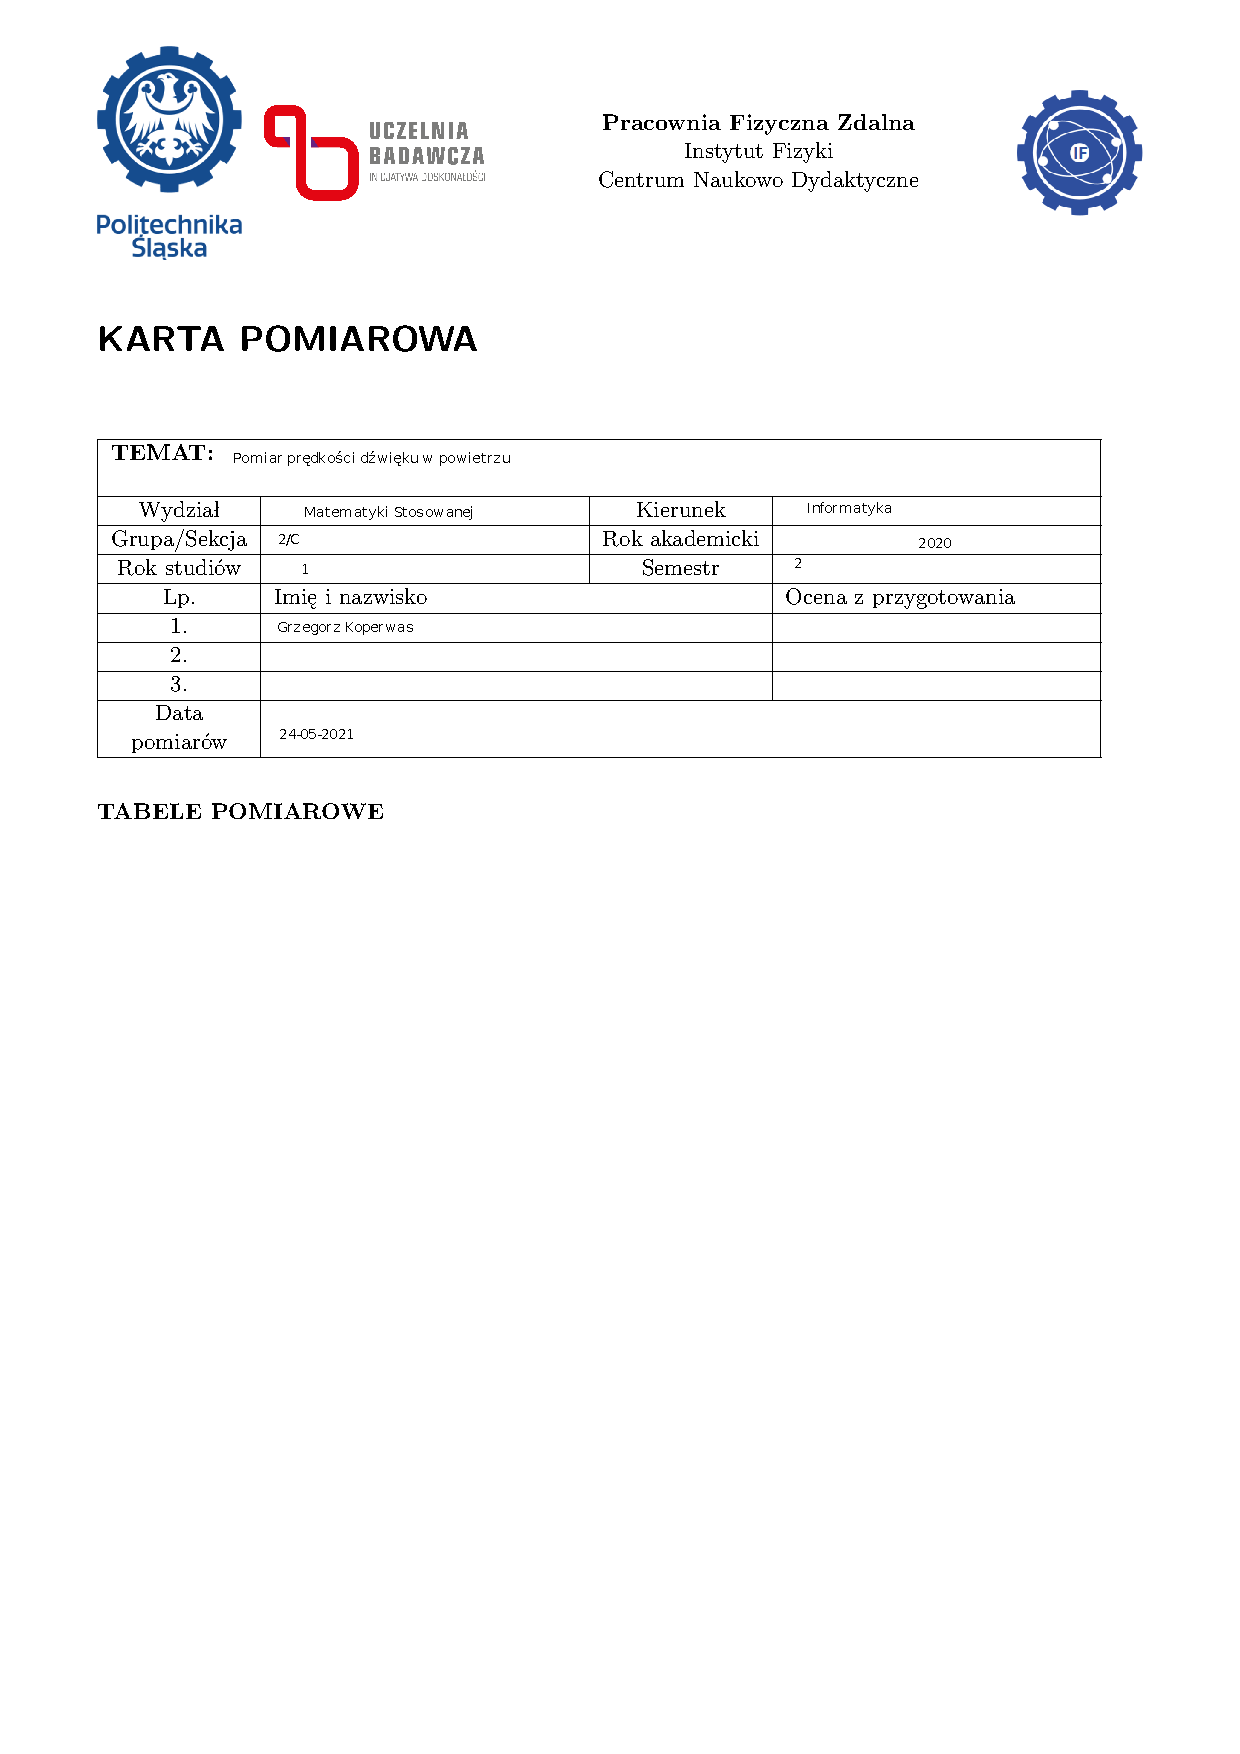
\includepdf[pages=-]{PFZ-KartaPomiarowa.pdf}
\begin{table}
	\begin{tabular}{|l|l|l|l|}
		\hline
		$t_1 [s] \pm 0,001 s$	& $t_2 [s] \pm 0,001 s$ & $t_1 - t_2$ & v $\left[\frac{m}{s^2}\right]$ \\\hline\hline
6,915	& 6,885	& 0,030	& 333,333 	\\\hline
6,780	& 6,745	& 0,035	& 285,714 	\\\hline
6,112	& 6,118	& -0,006	& -1666,667 	\\\hline
6,805	& 6,757	& 0,048	& 208,333 	\\\hline
6,892	& 6,861	& 0,031	& 322,581 	\\\hline
7,783	& 7,755	& 0,028	& 357,143 	\\\hline
8,082	& 8,057	& 0,025	& 400,000 	\\\hline
8,413	& 8,371	& 0,042	& 238,095 	\\\hline
8,603	& 8,537	& 0,066	& 151,515 	\\\hline
7,678	& 7,597	& 0,081	& 123,457 	\\\hline\hline
5,274	& 5,283	& -0,009	& -666,667 	\\\hline
5,243	& 5,236	& 0,007	& 857,143 	\\\hline
5,082	& 5,085	& -0,003	& -2000,000 	\\\hline
4,852	& 4,836	& 0,016	& 375,000 	\\\hline
6,154	& 6,140	& 0,014	& 428,571 	\\\hline
5,416	& 5,404	& 0,012	& 500,000 	\\\hline
4,774	& 4,737	& 0,037	& 162,162 	\\\hline
5,129	& 5,108	& 0,021	& 285,714 	\\\hline
5,154	& 5,120	& 0,034	& 176,471 	\\\hline
4,325	& 4,307	& 0,018	& 333,333 	\\\hline
	\end{tabular}
	\centering
	\caption{Pomiary dla 5m}
\end{table}
$t_1$ Mierzone telefonem, $t_2$ mierzone laptopem.

\end{document}
